Vr beim Auto manufaktur
Bei der Auto Manufaktur werden sogenannte VTS (Virtual-Trainings-Systeme verwendet. Bei einem dies VTS sieht der Benutzer eine Virtuelle Welt, in der er das das Auto sehen und verändern kann, dabei kann der Benutzer Schrauben, Motoren, Sitze und so weiter einbauen wie und wo er möchte.
\\
\begin{figure}[!ht]
    \centering
    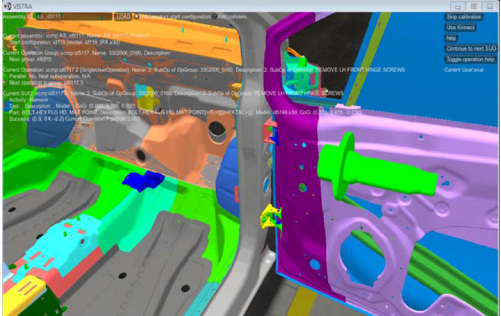
\includegraphics[width=1.0\textwidth]{images/Abbildung 4.png}
    \caption{\label{fig:Abbildung 4}Hier sieht man ein Beispiel dieser Virtuellen Welt durch das VTS VISTRA \cite{langley2016establishing}.\protect
    }
\end{figure}
\\
Damit VR-Training bei der Autoherstellung akzeptiert werden kann, muss es als nützliche und effektive Trainingsmethode anerkannt werden. Dazu haben \cite{langley2016establishing} eine Studie gemacht bei der folgendes als Ergebnis herauskam: „Diese Arbeit hat begonnen, die Effektivität und Effizienz des ersten Prototyps des VTS (Virtual-training-system) mithilfe objektiver und subjektiver Maßnahmen zu etablieren. Allerdings hat diese Studie auch eine Reihe von Problemen identifiziert, die im nächsten Entwicklungs- und Verbesserungszyklus berücksichtigt werden. \cite{langley2016establishing} “.
\\
\begin{figure}[!ht]
    \centering
    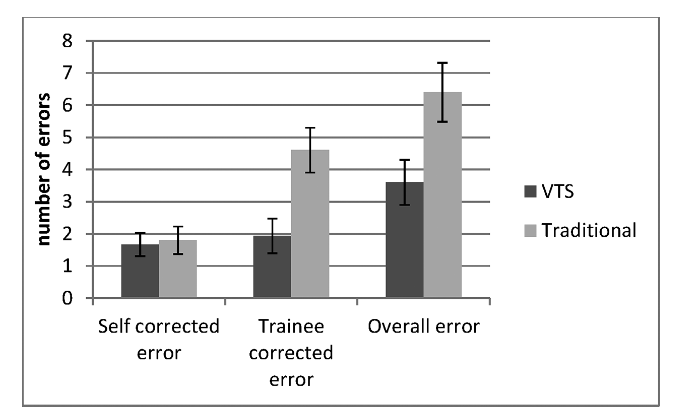
\includegraphics[width=1.0\textwidth]{images/Abbildung 5.png}
    \caption{\label{fig:Abbildung 5}In dieser Abbildung sieht man einen Vergleich von Ergebnissen der Studie von \cite{langley2016establishing}.\protect
    }
\end{figure}
\\
Hier werden die selbst-behobenen Fehler, vom Trainer behobene Fehler und die Insgesamten Fehler von Lehrlingen, die zu einem das VTS benutzt haben und zum anderen die traditionale Variante benutzt haben, gezeigt. Hier sieht man das bei dem VTS insgesamt nur halb so viele Fehler passiert sind und daraus kann man schließen, dass durch den VTS-Fehler besser ausgeschlossen werden können\cite{langley2016establishing}.
Im Bereich der Automanufaktur ist die VR-Technologie noch kaum angekommen, aber da wo es angekommen ist bietet es Vorteile. Daraus lässt sich schließen, dass auch in diesem überraschenden Bereich, die VR-Technologie immer mehr und mehr benutzt werden wird.
